\chapter{Security Measures}\label{chapter:security_measures}
\todoin{Short intro text here}
\todoin{Description: Enumerate the security features your application uses and which attacks each feature defends against (specify which features you implemented and which you borrowed/use from other libraries)}


\subsection{HTTPS with HSTS}

\subsection{SSL secure ciphers}
SSL ciphers are configured to the latest standards. As visible in \autoref{figure:ciphers1} and \autoref{figure:ciphers2}.
\begin{figure}[h!tbp]
	\centering
	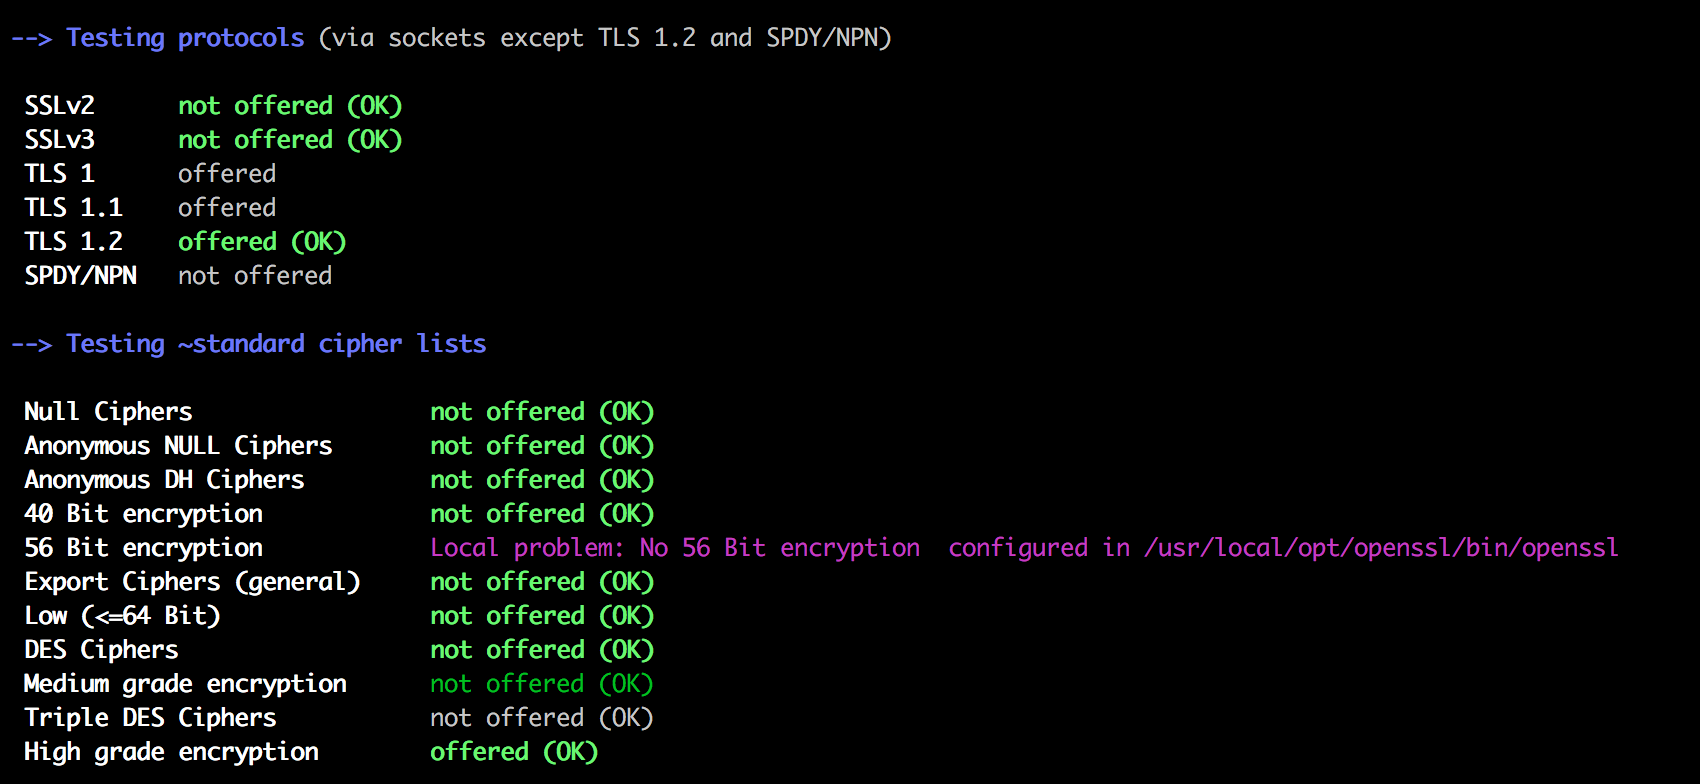
\includegraphics[width=\textwidth]{figures/ciphers1.png}
	\caption{Available SSL Ciphers}
	\label{figure:ciphers1}
\end{figure}
\begin{figure}[h!tbp]
	\centering
	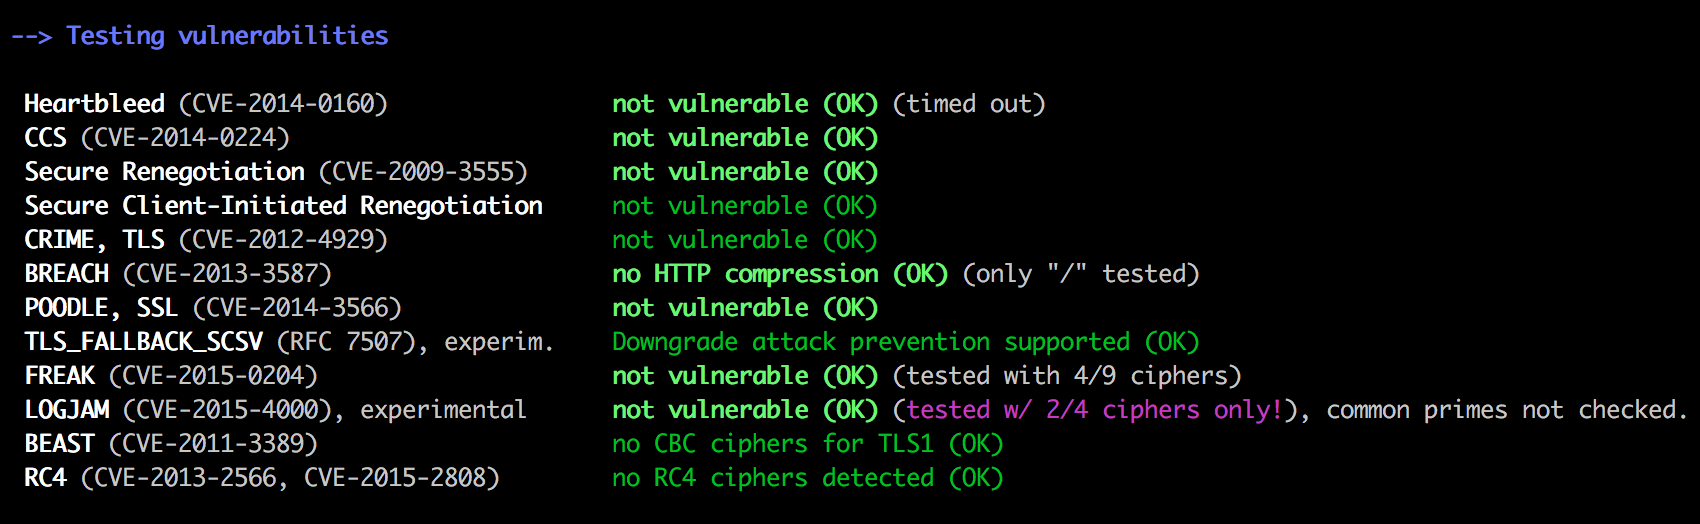
\includegraphics[width=\textwidth]{figures/ciphers2.png}
	\caption{No known SSL Vulnerabilities}
	\label{figure:ciphers2}
\end{figure}


\subsection{CSRF Tokens}

\subsection{Password reset with second factor}

\subsection{Lockout mechanism after failed password entries}

\subsection{Captcha}

\subsection{Balance calculated in database (Realtime concurrent transactions)}

\subsection{TANs in password protected PDFs}
